\documentclass{llncs}

\usepackage{url}
\usepackage{graphics}

\newcommand{\workingnote}[1]{}        % The version that hides the note.
%\newcommand{\workingnote}[1]{(**#1)}   % The version that makes the note visible.

\renewcommand\url{\begingroup \def\UrlLeft{<}\def\UrlRight{>}\urlstyle{tt}\Url}
\newcommand\emailaddr{\begingroup \def\UrlLeft{<}\def\UrlRight{>}\urlstyle{tt}\Url}

%\newif\ifpdf
%\ifx\pdfoutput\undefined
%   \pdffalse
%\else
%   \pdfoutput=1
%   \pdftrue
%\fi

\begin{document}

%% Use dvipdfm instead. --DH
%\ifpdf
%  \pdfcompresslevel=9
%  \pdfpagewidth=\the\paperwidth
%  \pdfpageheight=\the\paperheight
%\fi

\title{Mixminion: Design of a Type III Anonymous Remailer}

% Removed for anonymous review
% 
% \author{George Danezis\inst{1} \and Roger Dingledine\inst{2} \and David Hopwood\inst{3}
%         \and Nick Mathewson\inst{4}}
% \institute{Cambridge University
% \email{\emailaddr{george.danezis@cl.cam.ac.uk}}
% \and
% The Free Haven Project
% \email{\emailaddr{arma@mit.edu}}
% \and
% Independent consultant
% \email{\emailaddr{david.hopwood@zetnet.co.uk}}
% \and
% The Free Haven Project
% \email{\emailaddr{nickm@alum.mit.edu}}}
\author{Name of Author(s)}
\institute{Name of Institute(s)}


\maketitle
\pagestyle{empty} 
  
\begin{abstract}

We present Mixminion, a message-based anonymous remailer protocol that
supports secure single-use reply blocks. Mixminion reply messages are
indistinguishable from forward messages, allowing forward and reply
messages to share
the same anonymity set. We add directory servers that allow users to
learn public keys and performance statistics of participating remailers,
and we describe nymservers that allow users to maintain long-term
pseudonyms using single-use reply blocks as a primitive. Our design
integrates link-level encryption between remailers to provide
forward anonymity. Mixminion brings together the best solutions from
previous work to create a conservative design that protects against most
known attacks.

%Because many of our design choices impact anonymity in surprising ways,
%we include careful discussion of the anonymity implications of each step.

\end{abstract}

\noindent \textbf{Keywords:} anonymity, MIX-net, peer-to-peer, remailer, nymserver, reply block

%%%%%%%%%%%%%%%%%%%%%%%%%%%%%%%%%%%%%%%%%%%%%%%%%%%%%%%%%%%%%%%%%%%%%%%

\section{Introduction}
\label{sec:intro}

Chaum first introduced anonymous remailer designs over 20 years ago
\cite{chaum-mix}. The research community has since introduced many new
designs and proofs
\cite{abe,web-mix,babel,flash-mix,realtime-mix,kesdogan,shuffle,hybrid-mix},
and discovered a variety of new attacks
\cite{back-traffic-analysis,langos02,disad-free-routes,desmedt,mitkuro,raymond00},
but the state of deployed remailers has changed remarkably little since
Cottrell published his Mixmaster software \cite{mixmaster-attacks} in 1994. 
Part of the difficulty in expanding the deployed remailer base is
due to the liability involved in running a remailer node on the Internet,
and part is due to the complexity of the current infrastructure ---
it is fairly hard to add new experimental features to the current software.

The Mixminion project aims to deploy a cleaner updated remailer design
in the same spirit as Mixmaster, with the goals of expanding
deployment, documenting our design decisions and how well they stand
up to all known attacks, and providing a research base for
experimental features. We describe our overall design in Section
\ref{sec:design}, including a new primitive called a \emph{single-use
reply block} (SURB).  Mixmaster provides no support for replies, but
instead relies on the older and less secure cypherpunk Type I remailer
design \cite{remailer-history}. By integrating reply capabilities into
Mixminion, we can finally retire the Type I remailer network.

We introduce link-level encryption with ephemeral keys to ensure forward
anonymity for each message. We also provide flexible delivery schemes ---
rather than just allowing delivery to mail or Usenet, we allow designers
to add arbitrary modules to handle incoming and outgoing messages. By
separating the core mixing architecture from these higher-level modules,
we can limit their influence on the anonymity properties of the system. We
go on in Section \ref{sec:dir-servers} to describe a design for directory
servers to track and distribute remailer availability, performance,
and key information, and then describe in Section \ref{sec:nymservers}
how to securely build higher-level systems such as nymservers using SURBs.

Mixminion is a best-of-breed remailer that uses conservative design
approaches to provide security against most known attacks. The overall
Mixminion project is a joint effort between cryptography and anonymity
researchers and Mixmaster remailer operators. This design document
represents the first step in peer review of the Type III remailer
protocol.

%%%%%%%%%%%%%%%%%%%%%%%%%%%%%%%%%%%%%%%%%%%%%%%%%%%%%%%%%%%%%%%%%%%%%%%

\section{Related Work}

\subsection{MIX-nets}

Chaum introduced the concept of a MIX-net for anonymous communications
\cite{chaum-mix}. A MIX-net consists of a group of servers, called
MIXes (or MIX nodes), each of which is associated with a public
key. Each MIX receives encrypted messages, which are then decrypted,
batched, reordered, and forwarded on without any information
identifying the sender. Chaum also proved the security of MIXes
against a \emph{passive adversary} who can eavesdrop on all
communications between MIXes but is unable to observe the reordering
inside each MIX.

Current research directions on MIX-nets include ``stop-and-go'' MIX-nets
\cite{kesdogan}, distributed ``flash MIXes'' \cite{flash-mix} and their
weaknesses \cite{desmedt,mitkuro}, and hybrid MIXes \cite{hybrid-mix}.

One type of MIX hierarchy is a cascade.
In a cascade network, users choose from a set of fixed paths through
the MIX-net.
Cascades can provide greater anonymity against a large adversary:
free-route systems allow an adversary who owns many MIXes to use
intersection attacks to reduce the set of possible senders or receivers
for a given
% still not quite worded well. -RRD
message \cite{disad-free-routes}. On the other hand, cascades are more
vulnerable \cite{batching-taxonomy} to trickle attacks, where an attacker
targeting a specific message going into a MIX can manipulate the batch
of messages entering that MIX so the only unknown message in the batch
is the target message \cite{mixmaster-attacks,babel}.
MIX cascade research includes real-time MIXes \cite{realtime-mix} and
web MIXes \cite{web-mix}.

\subsection{Deployed Remailer Systems}

The first widespread public implementations of MIXes were produced by the
cypherpunks mailing list. These ``Type I'' \emph{anonymous remailers}
were inspired both by the problems surrounding the {\tt anon.penet.fi}
service \cite{helsingius}, and by theoretical work on MIXes. Hughes wrote
the first cypherpunks anonymous remailer \cite{remailer-history}; Finney
followed closely with a collection of scripts that used Phil Zimmermann's
PGP to encrypt and decrypt remailed messages. Later, Cottrell implemented
the Mixmaster system \cite{mixmaster}, or ``Type II'' remailers, which
added message padding, message pools, and other MIX features lacking
in the cypherpunk remailers. Note that Mixmaster does not include reply
functionality, so deployed remailer systems still use the less secure
long-term cypherpunk reply blocks.

At about the same time, Gulcu and Tsudik introduced the Babel
system \cite{babel}, a practical remailer design with many desirable
features. While it provides replies, they are only indistinguishable
from forward messages by passive observers; the MIX nodes can still
distinguish. Babel's reply addresses are multiple-use, making them less
secure than forward messages due to replay vulnerabilities. Babel also
introduces \emph{inter-MIX detours}, where nodes can rewrap a message
and send it through a few randomly chosen new hops --- so even the sender
cannot be sure of recognizing his message as it leaves the MIX.

%\subsection{Robustness}
%
%Previous work primarily investigates the \emph{robustness} of MIX-nets
%in the context of a distributed MIX system \cite{flash-mix}. A MIX
%is considered robust if it survives the failure of any $k$ of $n$
%participating servers, for some threshold $k$. This robustness is
%all-or-nothing: either $k$ servers are good and the MIX works, or they are
%not good and the MIX likely will not work.
%
%Robustness has been achieved primarily via zero-knowledge proofs of
%correct computation.  Jakobsson showed how to use precomputation to reduce
%the overhead of such a MIX network to about 160 modular multiplications
%per message per server \cite{flash-mix}, but the protocol was later
%found to be flawed \cite{mitkuro} by Mitomo and Kurosawa.  Desmedt and
%Kurosawa's alternate approach \cite{desmedt} requires many participating
%servers. Abe's MIX \cite{abe} provides \emph{universal verifiability} in
%which any observer can determine after the fact whether a MIX cheated,
%but the protocol is still computationally expensive. Neff recently
%made further efficiency improvements to universally verifiable mixing
%\cite{shuffle}.

\subsection{Remailer Statistics}

Levien's \emph{statistics pages} \cite{levien} track both remailer
capabilities (such as what kinds of encryption the remailer supports)
and remailer up-times (obtained by pinging the machines in question
and by sending test messages through each machine or group of
machines).  Such \emph{reputation systems} improve the reliability of
MIX-nets by allowing users to avoid choosing unreliable MIXes. The
Jack B Nymble 2 remailer client \cite{potato} and the Mixmaster 2.9
remailer allow users to import statistics files and can then pick
remailers according to that data. Users can specify minimum
reliability scores, decide that a remailer should always or never be
used, and specify maximum latency. Ongoing research on more powerful
reputation systems includes a reputation system for free-route
networks \cite{mix-acc} and another for MIX cascades \cite{casc-rep}.

%%%%%%%%%%%%%%%%%%%%%%%%%%%%%%%%%%%%%%%%%%%%%%%%%%%%%%%%%%%%%%%%%%%%%%%

\section{The MIX-net Design}
\label{sec:design}

Mixminion brings together the current best approaches for providing
anonymity in a batching message-based MIX environment. We don't aim
to provide low-latency connection-oriented services like Freedom
\cite{freedom} or Onion Routing \cite{goldschlag99} --- while those
designs are more effective for common activities like anonymous web
browsing, the low latency necessarily implies smaller anonymity sets
than for slower message-based services. Indeed, we intentionally
restrict the set of options for users: we provide only one
cipher suite, and we avoid extensions that would help an adversary
divide the anonymity set.

Mixminion uses the same general MIX-net paradigm as previous work
\cite{chaum-mix,mixmaster-attacks,babel}. The sender Alice chooses a
path through the network. She repeatedly ``onion'' encrypts her message,
starting with the last
MIX in her path, and sends the onion to the first MIX in her path. Each
MIX unwraps a single layer of the onion, pads the message to a fixed
length (32KB in our current design), and passes the result to the
next MIX. We describe the behavior of the last MIX in
Section \ref{subsec:delivery-modules}.

% A bit more detail about what is contained in the header: -George

Headers addressed to each intermediate mix are encrypted using RSA
%RSA-OAEP \cite{PKCS1}
% IMO we should use OAEP+. -DH
and are of 128 bytes each. They contain a secret addressed
to the node that can be used to generate padding and decrypt the rest
of the message. They also contain the address of the next node to 
which to message should be forwarded along with its expected signature 
key fingerprint. In order to frustrate tagging attacks (as described later
in the paper) the sub-header also contains a hash of the header that
should be checked. 

% This last paragraph assumes that the audience already knows the
% material well enough to know that Alice encrypts each layer with the
% appropriate MIX's public key. Is this assumption safe -Nick

While Mixminion protects against known \emph{traffic analysis} attacks
(where an adversary attempts to learn a given message's sender or
receiver \cite{rackoff93cryptographic,raymond00}), we do not fully
address \emph{traffic confirmation} attacks. In a traffic confirmation
attack, the adversary treats the MIX network as a black box and
observes the behavior of senders and receivers. Over time, he can
intersect the set of senders and receivers who are active at certain
times and learn who is sending and receiving which messages
% Really?  I thought that an intersection attack told you who was
% talking with whom, not which messages were sent to whom.  I.e., Eve
% can learn that Alice is sending messages to Bob and Carol, but
% can't be certain which messages were meant for whom. -Nick
% But if we further intersect to learn that the messages on Tuesday
% are for Bob and those on Wednesday are for Carol, ... -RRD
\cite{langos02}. Good dummy traffic designs may eventually address the
intersection attack, but for now it remains an open problem.

We choose to drop packet-level compatibility with Mixmaster and the
cypherpunk remailer systems, in order to provide a simple extensible
design. At the same time, we provide a new feature: a reply block
mechanism that is as secure as forward messages.

Reusable reply blocks, such as those in the cypherpunk remailer, are a
security risk --- by their very nature they let people send multiple
messages through them.  These multiple messages can easily be used to
trace the recipient's path: if two incoming batches both include a
message to the same reply block, then the next hop must be in the
intersection of both outgoing batches.  To prevent these replays,
Mixminion therefore provides only \emph{single-use} reply
blocks. Further, the Mixminion protocol makes reply messages
indistinguishable from forward messages, allowing forward and reply
messages to share the same anonymity set.

\subsection{Batching Strategy and Network Structure}
\label{subsec:batching}

[This subsection is draft/experimental/controversial. Don't pay much
attention to it yet.]
% This needs more work. I hadn't realised how close we were to the
% deadline, but I'll commit it anyway for now. -DH

Ideal security for a MIX-net is achieved when each message leaving the
network could correspond to any message entering the network during a
period approximately equal to the maximum network latency, and vice-versa.

This ideal is not achieved by protocols like Mixmaster that use random
delays [[explain why]].
If such networks also use free routes, they are subject to attacks
described in \cite{disad-free-routes}. [[summarize them]]

To both maximize anonymity sets and prevent the above attacks, we
propose to use a strategy called {\em synchronous batching}.
The network has a fixed {\em batch period}, $t_{batch}$, which is closely
related to the maximum desired latency; a typical value could be 24 hours.
Messages entering the network in each batch period are queued until
the beginning of the next period. They are then sent through the MIX-net
synchronously, at a rate of one hop per {\em hop period}. All paths are
a fixed length $n$ hops, so that if no messages are dropped, the messages
introduced in a given batch will progress through their routes in
lock-step, and will all be transmitted to their final destinations $n$
hop periods later.

The latency is between $nt_{hop}$ and $t_{batch} + nt_{hop}$, depending
on when the message was submitted.

The set of messages sent to a node in a given hop period is called a
mini-batch, to distinguish it from the set of messages being sent
through the network as a whole. [[need better name?]]

[[Messages are tied to a given time period so that they cannot be delayed.
Explain why this prevents the attacks in [disad-free-routes], even
for free-route networks. Also explain why we need to use a hybrid
free-route/cascade approach (otherwise the anonymity set is limited by
the bandwidth that can be handled by a single cascade).]]

Define the {\em width}, $w$ of a MIX network using synchronous batching to
be the number of nodes that simultaneously process messages in each
hop period. (If this is not constant, we can still talk about the
maximum, minimum and mean width.)

An important constraint on the network structure is the maximum
bandwidth (traffic in unit time) through any given node.
Assume that sending a message over a single hop consumes a fixed
amount of network traffic; we can then use that as the unit for
traffic.

Let $T_{batch}$ be the expected throughput in a single batch period,
i.e. the number of messages that go through the network in a batch.

We can give nodes the maximum opportunity to make use of the available
bandwidth by setting $t_{hop} \simeq t_{batch}/n$.

%If the available nodes were used optimally (this is a big if),
%the bandwidth required through each node in this simplified case
%will be $\frac{T_{batch}}{wt_{hop}} = \frac{nT_{batch}}{wt_{batch}}$.

For any particular network structure, bandwidth constraints, and
assumed traffic levels, it is straightforward to calculate the
minimum width of the network, and therefore the maximum sizes of
mini-batches.

For example in the limiting case $w = 1$, the network consists of a
single MIX cascade (this is the situation considered in Section 7.1
of \cite{babel}).

Let $N$ be the number of nodes in the network. An interesting case
is $w = n = N$; in that case we could use a set of $N$ cascades
arranged as a Latin square.\footnote{[[define Latin square]]}
This ensures that all nodes make full use of the available bandwidth;
however it gives users no choice in the set of nodes used.

In practice, there are other considerations beside maximizing the
size of mini-batches:

\begin{enumerate}
\item reliability
\item giving users a choice of node sets?
\item anything else?
\end{enumerate}

Further analysis of the trade-offs will be needed before choosing a
final network structure. Note that a planned structure, where each
users' software follows the plan consistently when constructing
routes, will generally be able to achieve stronger and more easily
analysed security properties than less constrained approaches.

\subsection{Replies}
\label{subsec:replies}

The rest of this section describes the mechanism for secure replies,
including some new attacks and how we defeat them. Mixminion's reply
model is in part inspired by BABEL \cite{babel}, as it requires the
receiver of a reply block to keep no other state than its secret keys,
in order to read the reply.  All the secrets that are required in
order to strip the layers of encryption are derived from a master
secret contained in the last header of the single use reply block that
the creator of the block addresses to themselves and encrypt under
their own public key.

\subsection{Indistinguishable replies}
\label{subsec:header-swap}

By making forward messages and replies indistinguishable, we prevent an adversary
from dividing the message anonymity sets into two classes. In particular,
if replies are infrequent relative to forward messages, an adversary who controls
some of the MIXes can more easily trace the path of each reply:  even
though the batches may be large, the number of replies in each batch
will be quite small.

Having indistinguishable replies, however, creates new attacks.  In
Mixmaster, senders ensure message integrity by including a hash of
the entire message in each hop of the header.  Each MIX in the path
checks the integrity of the header and payload, and drops the message
immediately if it has been altered.  But in Mixminion, since the
author of a reply block is not the one writing the payload, this
hash checking can't be used in replies. Therefore, since we choose to make
forward messages and replies indistinguishable, we cannot include
hashes for forward messages either. This choice introduces a new class
of attacks known as \emph{tagging attacks}, which we discuss in more
detail in Section \ref{subsec:tagging}.

Mixminion allows Alice to send messages to Bob in one of three ways:

\begin{enumerate}
\item \textbf{Forward} messages where only Alice remains anonymous.
\item \textbf{Direct Reply} messages where only Bob remains anonymous.
\item \textbf{Anonymized Reply} messages where both Alice and Bob
   remain anonymous.
\end{enumerate}

We require parties that benefit from anonymity properties to run dedicated
software.  Specifically, senders generating forward messages must be able
to create onions, and receivers must be able to create reply blocks
and unwrap messages received through those reply blocks. Other parties,
such as those receiving forward messages and those sending direct reply
messages, do not need to run new software. (For example, the quoting
performed by ordinary mail software can be used to include the reply
block in a direct reply; this is sent to a node at the SMTP Reply-To:
address, which extracts the reply block and constructs a properly
formatted onion.)

% Do we ever say how to send a reply without software? -Nick
% Nope. We're just bluffing. Is that ok? -RRD
% We're not bluffing.  George used to have a way, but we haven't
%   mentioned it here.  Should we?  -Nick
% We do now. -DH

We divide a message's path into two \emph{legs}, and split the header
into two equal-size subheaders, each corresponding to a single leg.
Each hop contains a hash of the subheader it's a part of, so we can do
integrity-checking of the path (but not the payload) within each leg.
Each hop also contains a symmetric key, which is used to derive a
decryption key for decrypting the rest of the message. The MIX also
derives a padding seed from this master key. It uses this padding seed
to place
predictable padding at the end of the subheader, so the hash will
match even though each hop must regrow the subheader to maintain
constant length.

For forward messages, Alice provides both legs; for anonymous replies, Alice
uses Bob's reply block as the second leg, and generates her own path
for the first leg.  To send a direct reply, Alice can use an empty
first leg, or send the reply block and message to a MIX that can wrap
them for her.

When Alice creates her message, she encrypts the second subheader
with a hash of her payload (she also does the usual layered onion
encryptions). Alice's message then traverses the MIX-net as normal (every
hop pulls off a layer, verifies the hash of the current subheader,
and puts some junk at the end of the subheader), until it gets to a
hop that is marked as a \emph{crossover point}. This crossover point
performs a ``swap'' operation: it decrypts the second subheader with
the hash of the current payload, and then swaps the two subheaders. The
swap operation is detailed in Figure 1 --- specifically, the normal
operations done at every hop are those above the dotted line, and the
special operations performed only by the crossover point are those below
the dotted line.  We use a variable block size block cipher named BEAR
\cite{BEAR} as our encryption and decryption primitive.  BEAR offers
the property that if any bit of the encrypted material is changed, the
decryption will look like random bits. We can use BEAR in a mode where
decryption and encryption are equivalent, by using the same key for
both of its hash steps. See Section \ref{subsec:tagging} for a discussion of
% ``Both hash steps''?  We never mention Bear's hash steps... -Nick
% True. Does adding 'its' help? -RRD
% Adding 'of' helps more for me.  Also, doesn't George once have a
% source for this? -Nick
how this all-or-nothing encryption approach helps protect against tagging.


\begin{figure}
\begin{center}
\resizebox{10cm}{!}{\includegraphics{SWAP.eps}}
\caption{The operations required by the ``swap'' method} 
\end{center}
\end{figure}


\subsection{Defenses against tagging attacks}
\label{subsec:tagging}

% We never define what a tagging attack is. -Nick
% Yes we do. This following paragraph does, give or take. Should
%   we say more? -RRD
% We never actually said that the attack described is a tagging
%   attack.  

Without the crossover point, an adversary could mount a \emph{tagging
attack} by modifying (``tagging'') the payload of a forward message as
it leaves Alice, and recognizing it later when it reaches Bob.
Specifically, if our encryption mechanism were an ordinary
counter-mode cipher, he might alter a specific byte in the payload of
a message entering the MIX-net. Since many of the outgoing messages
will be in part predictable (either entirely plaintext, or with
predictable PGP header material), the adversary can later observe
messages exiting the MIX-net and look for payloads that have a
corresponding anomaly at that byte.

% BEAR is a pretty exotic mode, and CTR is the only alternative we
% dismiss.  I think we shold point out =someplace= why we can't use
% CBC or anything else that isn't symmetrically good for encryption
% and decryption.  -Nick

We use BEAR as our encryption primitive to minimize the amount of
information an adversary can learn from tagging. If he tags a message
leaving Alice, the payload will be entirely random when it reaches
Bob.  Thus, an adversary who tags a message can at worst turn the
corresponding payload into trash.  
%%Thus if he tags more than one message in the entire MIX-net, he
%%learns only one bit from each tagged message, so he cannot distinguish
%%the tagged messages. 
% I think that the above sentence raises more objections than it 
% addresses; thus, I'm omitting it.  The real security comes from the
% crossover step as described below.  Without the crossover
% decryption, BEAR is insufficient, and one bit is too much. -Nick
Nevertheless, this may still allow an adversary to
break anonymity in some cases.

We briefly considered introducing \emph{cover-trash} to frustrate
these tagging attacks; but that problem is as complex as the dummy
traffic problem. Instead, we use the decryption-by-hash-of-payload step at the
crossover point to prevent the attacker from learning information from
tagging attacks.  Specifically, our solution falls into several cases:

\begin{itemize}
\item Forward messages: if the message is tagged during the first leg,
the second subheader is unrecoverable, and so the adversary cannot
learn the intended destination of the message. If the message is tagged
during the second leg, then the first leg has already provided anonymity,
and so the adversary cannot learn the sender.
\item Direct reply messages: since the encryption algorithm is equivalent to
decryption, the payload is effectively \emph{encrypted} at each step
% Maybe this  should say, ``Since the decryption algorithm provides
% secrecy equivalent to encryption''? -Nick
along a reply block. Only the recipient can learn, after peeling off
all layers of encryption, whether the message has been tagged. Thus
tagging attacks are useless against reply messages.
\item Anonymized reply messages: as with forward messages, if the first leg
is tagged the second subheader is unrecoverable --- so an adversary will
never learn that the message was addressed to a reply block. And as with
reply messages, only the recipient can learn if the second leg is tagged.
\end{itemize}

While direct reply messages do not need a crossover point in the path
(the adversary can never observe his tag), forward messages still need a
crossover point to prevent end-to-end tagging. But since the first leg
either provides sufficient anonymity or destroys the information about
the second leg, the second leg in a forward message can be very short.
At the extreme, the first hop in the second subheader could directly
specify the message recipient. But since the choice of crossover point
can still reveal information about the intended recipient (for instance,
some MIXes may only allow outgoing mail to local addresses; if such a
node gets a crossover message that has been trashed, it might guess
that the recipient is one of the local addresses), we recommend that
the second leg be at least a few hops long.
% The parenthetical above resists my attempts to remove or shorten
% it.  Can anybody else shorten or strike it? -Nick

Replies are indistinguishable at every hop from forward messages. Even the
crossover point cannot know if it's processing a reply or forward message.
The protocol doesn't allow a MIX to know its location in the path (other
than the exit node), or the total length of the route.

\subsection{Multiple-message tagging attacks}
\label{subsec:multi-tagging}

The above design is still vulnerable to a subtle and dangerous
attack. If Alice sends a group of messages along the same path, the
adversary can tag some of those message as they leave Alice, recognize
the pattern (number and timing of tagged and untagged messages) at the
crossover point, and observe where the untagged ones go (if he built
the second leg himself, as in an anonymized reply, he can recognize
it immediately).

With some assumptions about our adversary, we can reduce
this attack to a traffic confirmation attack we're already willing to
accept: when Alice sends a bunch of messages, the adversary can count
them and look for the pattern later. He can also drop some of them and
look for resulting patterns.

The adversary can only recognize a tag if he happens to own the crossover
point that Alice chooses.
Therefore, Alice picks $k$ crossover points for her $n$
messages;\footnote{
  We can prevent the adversary from using divide-and-conquer on Alice's
  batches if Alice uses a hybrid path starting with a short cascade ---
  so even if the adversary tags a subset of the messages he doesn't know
  (unless he owns the whole cascade) where the tagged messages went.
}
an adversary who wants to match a tag signature with certainty would
have to own all $k$ crossover points.  (And even then, it seems harder
because the subsets of her messages would overlap with subsets of
messages from other senders.)

% The argument above seems a little handwavy to me.  We should either
% expand it to say why the adversary needs certainty to mount the
% multiple-messages attack, or express less confidence in it.  I'm
% taking the latter route below, and changing ``is infeasible''
% to ``seems infeasible''  -Nick

The key here is that when the adversary doesn't own a given crossover
point, tagging messages destined for that crossover is equivalent to
dropping them.  The crossover point in question simply doesn't deliver
the message to the second leg. Therefore, if the adversary doesn't own
most of the crossover points that Alice chooses, a successful
multiple-message tagging attack seems infeasible.  We leave a security
analysis of this multiple-paths approach to future work.
% reference section \ref{sec:choosing-paths} when/if we write it -RRD

\section{Related design decisions}

In this section we discuss how we are using
link-level encryption with ephemeral keys to provide forward anonymity,
message types and modules to handle different types of messages, and
exit policies for advertising what delivery options a node will provide.

\subsection{Link-level encryption and what it gets us}
\label{subsec:link-encrypt}

Unlike remailer Types I and II that used SMTP \cite{SMTP} (i.e. ordinary
Internet e-mail) as their underlying transport mechanism, Mixminion
clients and nodes communicate using a forward secure encrypted channel
based on TLS \cite{TLS}.  
TLS allows the establishment of an encrypted tunnel using ephemeral
Diffie-Hellman keys. In order to guarantee that the receiving end is
the one intended by the creator of the anonymous message, the
receiving node can sign the ephemeral key. As soon as a session key
has been established, the parties destroy their Diffie-Hellman keys
and begin sending messages through the tunnel. After each message, the
parties perform a standard key update operation to generate a fresh
key, and delete the old key material.  Key updates don't require any
asymmetric encryption techniques, so they are relatively fast.

% Do we want to specify how much of the above happens with TLS
% Handshake/ChangeCipherSpec packets, and how much happens within the 
% application data?  I =believe=[*] that TLS can do all of the above with 
% standard stuff; do we want to use TLS vocabulary to convince
% people? 
%
%  [*]My only reservation is doing key updates without assymetric
%  encryption.  I need to doublecheck that such an operation is really 
%  specified in the RFC.                               -Nick
%  It is: the server can send a HelloRequest or the client a
%  ClientHello at any time. -DH.


% Also, do we want to specify a required level of encryption?  It
% would be pretty useless if we allowed export or null ciphers
% suites.
%
% One of these modes (specified in ietf-tls-ciphersuite-03.txt) is
% probably best for us:
%             (A)   ``DHE-DSS-AES128-SHA''
%             (A)   ``DHE-RSA-AES128-SHA''
%             (B)   ``ADH-AES-128-SHA''
%             (A)   ``DHE-DSS-AES256-SHA''
%             (A)   ``DHE-RSA-AES256-SHA''
%             (B)   ``ADH-AES256-SHA''
% I'm not sure, though, whether we want one of the cert-based ones (A)
% or one of the the anon-server ones. (B) -Nick

The purpose of link-level encryption is to provide forward secrecy: 
% link-level, *not* link-layer. link-layer is a layer-2 OSI thing.
% saying that our transport level protocol uses link-layer encryption
% makes no sense. -RRD
after the keys
have been deleted, not even the
nodes that exchange messages can decrypt or recognize messages
that might have been intercepted on the links. This makes it
impossible to comply with decryption notices that might be served in
some jurisdictions.  
It also forces adversaries to 
corrupt and control nodes in order trace
a forward anonymous communication by requesting nodes to decrypt
it. 
% In advance, or later?  I'm not clear what the above sentence is
% saying. -Nick
(Reply blocks can still be used for this purpose.)  Even if an
attacker manages to get hold of the session key at a particular point
they would have to observe all subsequent traffic to be able to update
their key appropriately.

The encrypted channel offers only limited protection against traffic
analysis. Encrypted links between honest nodes prevent an adversary
from recognizing even his own messages; but without link padding, he
can still measure how much traffic is being transmitted.

As a fringe benefit, using a separate link-level protocol makes it
easier to deploy relay-only MIXes --- such nodes simply omit SMTP
support.  (See Section \ref{subsec:delivery-modules} below.)
% Credit for the above point goes to Len.

\subsection{Message types and delivery modules}
\label{subsec:delivery-modules}

Once a Mixminion packet reaches the final MIX in its path, it must
either be delivered to its intended recipient, or dropped if it's an
intra-network dummy message. In order to support different kinds of
delivery, the header includes a type code for the action to be taken
to deliver the message.  A few types --- such as `dummy', `SMTP', and
`local delivery' --- are specified as a part of the Mixminion
standard.  Others may be added by future extensions, in order to
implement abuse-resistant exit policies (see Section
\ref{subsec:exitpolicies}), to administer nymservers (see Section
\ref{sec:nymservers}), to publish anonymously to Usenet, to relay
messages to older remailers, or to support other protocols.

Nearly all delivery methods require additional information beyond the
message type and its payload.  The SMTP module, for example, requires
a mailbox.\footnote{A {\it mailbox} is the canonical form of the
``{\tt user@domain}'' part of an e-mail address. Mixminion uses only
mailboxes in the protocol, because the display name and comment parts
of an e-mail address could potentially be different for senders who
have obtained an address from different sources, leading to smaller
anonymity sets.}
In our current design, this information is placed
in a variable-length annex to the final header.

%\footnote{It must be
%in the header, since putting delivery information in the payload would
%prevent people from creating SURBs that can be delivered by SMTP.
%On the one hand, under the ``header swap'' method described in
%\ref{subsec:header-swap}, the all-or-nothing property of BEAR prevents
%the generator of a reply block from putting any information in the
%payload.  On the other hand, under the ``distinguish replies'' method
%in \ref{subsec:distinguish-replies}, the delivery information would
%create a portion of the payload that the final node could
%distinguish from random garbage, thus allowing a tagging attack
%against the reply block.}.
%
% See my messages of April 9 and 10 titled ``SMTP service'' for a more
% detailed version of the above argument. -Nick
%
% Should we say _why_ it's undesirable to force reply recipients to
% run local nodes?  [My answer is (A) that some people (such as human
% rights activists using internet cafes) want to get replies, but
% don't have persistent net connections, (B) that Mixmaster
% supports it, and not doing so would be a step backwards, and (C)    
% that there's not much reason not to.]    -Nick
%%%%%%
% The above footnote and comments comment, deleted by RRD, re-added by
% DH, is of historical interest only. :)  Nonetheless, it's still a
% subtle point.  Mixmaster  puts the delivery info in the payload; 
% someplace, perhaps in a different  document, we should explain why 
% we don't.  -Nick

The types each MIX supports are described in a \emph{capability block},
which also includes the MIX's address, long-term (signing) public key,
short-term key (for use in header encryption), and batching strategy.
MIXes sign these capability blocks
and publish them on directory servers (see Section \ref{sec:dir-servers}).
Clients download this information from the directory servers.

% Is all of the stuff above really in the caps block?  Or do we break
% the volatile part (short-term key) from the nonvolatile part? -Nick
%
% I think they should be in the same block, although probably
% "capability block" isn't a good name for it. Capabilities should
% also be able to change without losing identity/reputation, and
% there would be no point in having two separate update mechanisms. --DH

The possibility of multiple delivery methods doesn't come free: their
presence may fragment the anonymity set.  For example, if there were five
ways to send an SMTP message to Bob, an attacker could partition Bob's
incoming mail by guessing that one of those ways is Alice's favorite.
An active attacker could even lure users into using a compromised
exit node by advertising that node as supporting a
rare but desirable delivery method.

We claim that these attacks do not provide an argument against
extensibility \emph{per se}, but rather argue against the proliferation
of redundant extensions, and against the use of rare extensions.  

\subsection{Exit policies and abuse}
\label{subsec:exitpolicies}

One important entry in a node's capability block is its \emph{exit
policy}. Exit abuse is a serious barrier to wide-scale remailer deployment
--- rare indeed is the network administrator tolerant of machines that
potentially deliver hate mail to the U.S. President.

On one end of the spectrum are \emph{open exit} nodes that will
deliver anywhere; on the other end are \emph{middleman} nodes that
only relay traffic to other remailer nodes and \emph{private exit}
nodes that only deliver locally. More generally, nodes can set
individual exit policies to declare which traffic they will let exit
from them, such as traffic for local users or other authenticated
traffic \cite{onion-discex00}.

Preventing abuse of open exit nodes is an unsolved problem. If
receiving mail is opt-in, an abuser can forge an opt-in request from
his victim. Indeed, requiring recipients to declare their interest
in receiving anonymous mail is risky --- human rights activists in
Guatemala cannot both sign up to receive anonymous mail and also retain
plausible deniability.\footnote{
  Compare with the 1965 U.S. Supreme Court case Lamont v. Postmaster
  General (381 U.S. 301), where the Post Office would detain mail it
  deemed to be `communist political propaganda' and instead send a form
  to the addressee telling him to send back the signed form if he wanted
  to receive such mail. The government maintained a list of citizens
  who had filled out these forms.
} Similarly, if receiving mail is opt-out, an abuser can deny service
by forging an opt-out request from a legitimate user. We might instead
keep the mail at the exit node and send a note to the recipient
telling them how to collect their mail; but this increases
server liability by storing messages (see Section \ref{sec:nymservers}
below), and also doesn't really solve the problem.

Of course, a mixture of open and restricted exit nodes will allow the
most flexibility for volunteers running servers. But while a large number
of middleman nodes is useful to provide a large and robust network, the
small number of exit nodes still simplifies \emph{traffic confirmation}
(attacks where the adversary observes both a suspected user and the
network's exit nodes and looks for timing or packet correlations). The
number of available open exit nodes remains a limiting security parameter
for the remailer network.

\subsection{Replay prevention, message expiration, and key rotation}

Mixmaster offers rudimentary replay prevention by keeping a list of recent
message IDs. To keep the list from getting too large, it expires entries
after a user-configurable amount of time. But if an adversary records
the input and output batches of a MIX and then replays a message after
the MIX has forgotten about it, the message's decryption will be exactly
the same. Thus, Mixmaster does not provide the forward anonymity that we want.

Chaum first observed this attack in \cite{chaum-mix},
but his solution (which is proposed again in Babel\footnote{
  Actually, Babel is vulnerable to a much more direct timestamp attack:
  each layer of the onion is timestamped with ``the number of seconds
  elapsed since January 1, 1970 GMT, to the moment of message composition
  by the sender.'' Since the number of people composing a message on
  the same second will likely be small, an adversary owning a MIX at the
  beginning of the path and another at the end could trivially recognize
  a message.
}) --- to include in each message a timestamp that describes when that message
is valid --- also has problems. Specifically, it introduces a new class
of \emph{partitioning} attacks, where the adversary can distinguish and
track messages based on timestamps. If messages have short lifetimes,
legitimate messages may arrive after their expiration date and be
dropped. But if we specify expiration dates well after when we expect the
message to arrive, messages arriving near their expiration date will be
rare: an adversary can delay a message until near its expiration date,
then release it and trace it through the network.

% need to read stop & go mix paper here. -RRD

One way of addressing this partitioning attack is to add dummy traffic
so that it is less rare for messages to arrive near their expiration date;
but dummy traffic is still not well-understood. Another approach would
be to add random values to the expiration time of each MIX in the path,
so an adversary delaying a message at one MIX could not expect that it
is now near to expiring elsewhere in the path; but this seems open to
statistical attacks.

% Partitioning can be prevented completely using synchronous batching.
% Client software just needs to know the current time accurate to one
% batch period (e.g. one UTC day), and even if it gets that wrong, the
% message will just be dropped by the first honest node on the route.
% --DH
% True. We need to think more on the tradeoffs of the synchronous batching
% approach. It's definitely a good thing to mention. I've uncommented the
% below for now so readers can have a complete paper. -RRD

Mixminion provides a compromise solution that hopefully avoids many of
these problems while still providing forward anonymity. Messages don't
contain any timestamp or expiration information. Each MIX must keep
hashes of the headers of all messages it's processed since the last time
it rotated its key. MIXes should choose key rotation frequency based on
security goals and on how many hashes they want to store.

Note that this solution doesn't entirely solve the partitioning problem
--- near the time of a key rotation, the anonymity set of messages will
be divided into those senders who knew about the key rotation and used
the new key, and those who didn't.
Also note that while key rotation and link encryption (see Section
\ref{subsec:link-encrypt}) both provide forward security, their protection
is not redundant. With only link encryption, an adversary running
one MIX could compromise another and use its private key to decrypt
messages previously sent between them. Key rotation limits the window
of opportunity for this attack.

%%%%%%%%%%%%%%%%%%%%%%%%%%%%%%%%%%%%%%%%%%%%%%%%%%%%%%%%%%%%%%%%%%%%%%%

\section{Directory Servers}
\label{sec:dir-servers}

The Mixmaster protocol does not specify a means for clients to learn the
locations, keys, capabilities, or performance statistics of MIXes. Several
\emph{ad hoc} schemes have grown to fill that void \cite{levien}; here
% would be nice to cite some more. eg, are there key lists, etc? -RRD
we describe Mixminion directory servers and examine the anonymity risks
of such information services.

% ZZZZZZZZZZZZZ NM NM NM
%  what the heck is that, nick? :) -RRD

In Mixminion, a group of redundant directory servers serve current
node state.  It is important that these servers be synchronized and
redundant:  we lose security if each client has different information
about network topology and node reliability. An adversary who controls
a directory server could track certain clients by providing different
information, perhaps by listing only MIXes it controls or only
informing certain clients about a given MIX.

An adversary without control of a directory server can still exploit
differences among client knowledge. If Eve knows that MIX $M$ is listed
on server $D_1$ but not on $D_2$, she can use this knowledge to link
traffic through $M$ to clients who have queried $D_2$.  Eve can also
distinguish traffic based on any differences between clients who use
directory servers and those who don't; between clients who have up-to-date
listings and those who have old listings; and (if the directory is large
and so is given out in pieces) between clients who have different subsets
of the directory.
%  In fact, even if Eve does not know the exact
%difference between Alice's knowledge and Bob's, the presence of such a
%difference can aid her traffic analysis. [[CAN WE HAVE A CITE HERE?]]

So it is not merely a matter of convenience for clients to retrieve
up-to-date MIX information: if some client software supports a static
list of servers while other software is dynamic, this difference can
help an attacker distinguish their traffic. We must specify a directory
service as a part of our standard. Thus Mixminion provides protocols for
MIXes to advertise their capability certificates to directory servers,
and for clients to download \emph{complete} directories.\footnote{
  New advances in Private Information Retrieval \cite{malkin-thesis}
  may down 
  the
  road allow clients to efficiently and privately download a subset of
  the directory. We recommend against using the MIX-net to anonymously
  retrieve a random subset: an adversary observing the directory servers
  and given two hops in a message's path can take the intersection over
  recently downloaded directory subsets to guess the remaining hops in
  the path.}
Servers can work together to ensure correct and complete data by
successively signing certificate bundles, so users can be sure that a
given MIX certificate has been seen by a threshold of directory servers.

But even with if client knowledge is uniform, an attacker can mount a
\emph{trickle attack} by delaying messages from Alice at a compromised
node until the directory servers remove some MIX $M$ from their listings
--- he can then release the delayed messages and guess that any messages
still using $M$ are likely to be from Alice. An adversary controlling
many nodes can launch this attack very effectively. Thus clients
should download new information regularly,
but wait for a given time threshold (say, an hour) before using any
newly-published nodes. Dummy traffic to old nodes may also 
help thwart trickle attacks.

Directory servers compile node availability and performance information by
sending traffic through MIXes in their directories. In its basic form this
can be very similar to the current ping servers \cite{levien}, but in the
future we can investigate integrating more complex and attack-resistant
reputation metrics.   Even this reputation information introduces
vulnerabilities: for example, an adversary 
trying to do traffic analysis
% want to leave the above line in. Otherwise the reader will say
% "so? what does this get him?" -RRD
can get more traffic by gaining a high reputation \cite{mix-acc}. We can
defend against these attacks by building paths from a suitably large pool
of nodes \cite{casc-rep} to bound the probability that an adversary will
control an entire path; but there will always be a tension between giving
clients accurate and timely information and preventing adversaries from
exploiting the directory servers to manipulate client behavior.

%We do not currently specify a means to detect and blacklist misbehaving
%directory servers. Because the set of such servers is smaller and more
%static than the set of nodes, we have some hope for out-of-band detection.

%%%%%%%%%%%%%%%%%%%%%%%%%%%%%%%%%%%%%%%%%%%%%%%%%%%%%%%%%%%%%%%%%%%%%%%

\section{Nym management and single-use reply blocks}
\label{sec:nymservers}

Current nymservers, such as {\tt nym.alias.net} \cite{nym-alias-net},
maintain a set of (mailbox, reply block) pairs to allow users to
receive mail without revealing their identities. When mail arrives to
\emailaddr{bob@nym.alias.net}, the nymserver attaches the payload to
the associated
reply block and sends it off into the MIX-net. Because these nymservers
use the Type I remailer network, these reply blocks are \emph{persistent}
or \emph{long-lived} nyms --- the MIX network does not drop replayed
messages, so the reply blocks can be used again and again. Reply block
management is much simpler in this model because users only need to
replace a reply block when one of the nodes it uses stops working.

The Mixminion design protects against replay attacks by dropping
messages with repeated headers --- so its reply blocks are necessarily
single-use. There are a number of approaches for building nymservers
from single-use reply blocks.

In the simplest approach, nymservers keep a stock of reply blocks for
each mailbox, and use a reply block for each incoming message. As long
as the owner of the pseudonym keeps the nymserver well-stocked, no
messages will be lost.  But it is hard for the user to know how many
new reply blocks to send; indeed, under this approach, an attacker can
launch a DoS attack by flooding the mailbox to exhaust the available
reply blocks and block further messages from getting delivered.

A more robust design uses a protocol inspired by e-mail retrieval
protocols such as IMAP \cite{IMAP} or POP \cite{POP3}:
messages arrive and queue at the nymserver, and the user periodically
checks the status of his mail and sends a sufficient batch of reply
blocks so the nymserver can deliver that mail. 
% Actually, isn't this more similar to POP? -Nick
% Yes, it is. We want to make sure the messages don't get deleted
% until we confirm we've gotten them. (is this even true? or do we
% just accept that some will get lost in the network.) But other
% than a difference in a the transport layer, you're right, it sounds
% like pop. -RRD
In this case, the nymserver doesn't need to store any reply blocks.
The above flooding attack still works, but now it is exactly
like flooding a normal IMAP or POP mailbox, and the usual techniques (such as
allowing the user to delete mails at the server or specify which mails to
download and let the others expire) work fine. The user can send a set
of hashes or other indices to the server after successfully receiving
some messages, to indicate that they can now be deleted.

Of course, there are different legal and security implications for the two
designs. In the first design, no mail is stored on the server, but it must
keep valid reply blocks on hand. The second case is in some sense more
secure because the server need not store any reply blocks, but it also
creates more liability because the server keeps mail for each recipient
until it is retrieved. The owner of the pseudonym could provide a public
key that the nymserver uses to immediately encrypt all incoming messages,
to limit the amount of time the nymserver keeps plaintext messages.

The best implementation depends on the situations and preferences of
the volunteers running the nymservers. Hopefully there will be enough
volunteers that users can choose the model that makes them most
comfortable.

%%%%%%%%%%%%%%%%%%%%%%%%%%%%%%%%%%%%%%%%%%%%%%%%%%%%%%%%%%%%%%%%%%%%%%%

\section{Maintaining anonymity sets}

\subsection{Transmitting large files with Mixminion}

We would like to use Mixminion as a transport layer for higher-level
anonymity applications such as anonymous publication systems
\cite{freehaven-berk}, but much research remains before we can
provide security for users transferring large files over Mixminion.

Alice wants to send a large file to Bob; thus she must send many Mixminion
messages. Conventional wisdom suggests that she should pick a different
% can I get a \cite here? -RRD
path for every message, but an adversary that owns all the nodes in
\emph{any} of the paths could learn her identity --- without any work
at all. (Even an adversary owning a very small fraction of the network
can perform this attack, since the Mixminion message size is small.)

% Assuming Alice picks five nodes at random for
%each path, at 28k of data per packet (assuming no redundancy or overhead)
%an adversary owning only 1\% of the MIXes has a better than even chance
%of identifying Alice as soon as she sends her fourteen packet. By the
%time she sends message 92 (meaning her file is roughly 2.5 megabytes),
%Alice has a less than 1\% chance of keeping her anonymity.

Alice seems more likely to maintain her unlinkability by sending all the
messages over the same path. On the other hand, a passive adversary can
still watch the flood of messages traverse that path. We must hope the
honest nodes will rearrange and obfuscate streams of messages enough to
foil these attacks. The multiple-message tagging attacks described in
Section \ref{subsec:multi-tagging} make the situation even more dangerous.

A compromise approach is to pick a small number of paths and use them
together. Still, if the messages are sent all at once, it seems clear
we're going to need some really good cover traffic schemes before we
can offer security.

\subsection{Long-term nyms: how to choose paths for reply blocks}
\label{subsec:choosing-paths}

In fact, this same problem comes up when the owner of a pseudonym is
downloading his mail from a nymserver.

Cue for David Hopwood's discussion, somewhere around here. Feel free
to muck this section up however it seems best.


%%%%%%%%%%%%%%%%%%%%%%%%%%%%%%%%%%%%%%%%%%%%%%%%%%%%%%%%%%%%%%%%%%%%%%%

%\section{Attacks and Defenses}
%\label{sec:attacks}
%
%[Do something akin to pages 13-15 of
%\url{http://freehaven.net/doc/casc-rep/casc-rep.ps}.]
%
%\subsection{MIX attacks}
%\label{subsec:mix-attacks}
%
%%\begin{description}
%Replay attack
%Message delaying
%Message dropping
%Tagging
%n-1 attack (trickle, flooding)
%intersection attack (short-term, long-term)
%textual analysis, etc
%%\end{description}
%
%\subsection{Exit-based attacks}
%\label{subsec:attacks-exitbased}
%
%Attack: use delivery method to partition anon set.
%Attack: use caps to partition anon set.
%
%[Need to expand this. -Nick]
%
%\subsection{Directory-based attacks}
%\label{subsec:attacks-dirbased}
%
%\begin{description}
%\item \emph{Compromize a directory server.} Identical directory listings
%  are served by a large group of servers, and signed by all.
%\item \emph{Lie to a directory server.}  Signed capability blocks, and
%  the fact that a MIX's signing key is its identity, prevent this
%  attack.
%\item \emph{Exploit differences in client directory knowledge.}  By
%  only updating directory information nightly; by urging client
%  software to pull updates as soon as possible after their release;
%  and by 
%\item \emph{Delay MIX packets until directory information changes.}
%  The delay in clients' using new information, along with dummy
%  traffic sent to de-listed destinations and expired keys, should
%  mitigate this attack. However, a complete solution remains an
%  open problem.
%\item \emph{Flood the directories with nonfunctional MIX entries.}
%  Availability statistics should mitigate this problem.  Nevertheless,
%  it remains an area of active research. \cite{mix-acc,casc-rep}
%[[WHAT OTHER DIRECTORY ATTACKS?]]
%\end{description}
%%\item \emph{X} Y.

%%%%%%%%%%%%%%%%%%%%%%%%%%%%%%%%%%%%%%%%%%%%%%%%%%%%%%%%%%%%%%%%%%%%%%%

\section{Future Directions}
\label{sec:conclusion}

This design document represents the first step in peer review of the
Type III remailer protocol. Many of the ideas, ranging from the core
design to peripheral design choices, need more attention:

\begin{itemize}
\item We need to analyze the proposed defense against the multiple-message
tagging attack.
\item We need more research on batching strategies that resist trickle
and flooding attacks \cite{batching-taxonomy} as well as intersection
free-route attacks \cite{disad-free-routes}.
% help, say that last phrase better -RRD
\item We need a more thorough investigation of multiple-message tagging
attacks, and an analysis of various ways of safely choosing paths when
sending many messages.
\item We claim that we use conservative techniques, but an all-or-nothing
variable-length block cipher is pushing it. Can we keep indistinguishable
forward messages and replies using a simpler design?
\item We need stronger intuition about how to improve security via
dummy messages.
\item We intend to draw up a more complete specification, which can lead
to implementation and deployment of the Mixminion design.
% We'll have to get another spec cobbled together before anybody can review
% this system thorougly.  Should we mention some place for people to
% get a more formal spec?  I wouldn't be able to review our system at
% the level that I'd want to without one.  -Nick 
\end{itemize}

%%%%%%%%%%%%%%%%%%%%%%%%%%%%%%%%%%%%%%%%%%%%%%%%%%%%%%%%%%%%%%%%%%%%%%%

%\section*{Acknowledgments} Removed for anonymous review.

%%%%%%%%%%%%%%%%%%%%%%%%%%%%%%%%%%%%%%%%%%%%%%%%%%%%%%%%%%%%%%%%%%%%%%%

\bibliographystyle{plain}

\bibliography{minion-design}

\end{document}

% Style guide:
%     'MIX', 'MIXes' (as noun)
%     'MIX-net'
%     'mix', 'mixing' (as verb)
%     'Mixminion'
%     'Mixmaster'
%     'middleman'  [Not with a hyphen; the hyphen has been optional
%         since Middle English.]
%     'nymserver'
%     'Cypherpunks Remailer'

